\documentclass[14pt]{extbook}
\usepackage{multicol, enumerate, enumitem, hyperref, color, soul, setspace, parskip, fancyhdr} %General Packages
\usepackage{amssymb, amsthm, amsmath, latexsym, units, mathtools} %Math Packages
\everymath{\displaystyle} %All math in Display Style
% Packages with additional options
\usepackage[headsep=0.5cm,headheight=12pt, left=1 in,right= 1 in,top= 1 in,bottom= 1 in]{geometry}
\usepackage[usenames,dvipsnames]{xcolor}
\usepackage{dashrule}  % Package to use the command below to create lines between items
\newcommand{\litem}[1]{\item#1\hspace*{-1cm}\rule{\textwidth}{0.4pt}}
\pagestyle{fancy}
\lhead{Progress Quiz 6}
\chead{}
\rhead{Version B}
\lfoot{4563-7456}
\cfoot{}
\rfoot{Summer C 2021}
\begin{document}

\begin{enumerate}
\litem{
Determine the vertical asymptotes and holes in the rational function below.\[ f(x) = \frac{6x^{3} -5 x^{2} -21 x -10}{12x^{2} +17 x + 6} \]\begin{enumerate}[label=\Alph*.]
\item \( \text{Vertical Asymptotes of } x = -0.75 \text{ and } x = -0.667 \text{ with no holes.} \)
\item \( \text{Vertical Asymptotes of } x = -0.75 \text{ and } x = 2.5 \text{ with a hole at } x = -0.667 \)
\item \( \text{Holes at } x = -0.75 \text{ and } x = -0.667 \text{ with no vertical asymptotes.} \)
\item \( \text{Vertical Asymptote of } x = -0.75 \text{ and hole at } x = -0.667 \)
\item \( \text{Vertical Asymptote of } x = 0.5 \text{ and hole at } x = -0.667 \)

\end{enumerate} }
\litem{
Determine the vertical asymptotes and holes in the rational function below.\[ f(x) = \frac{9x^{3} -15 x^{2} -74 x -40}{9x^{2} -9 x -10} \]\begin{enumerate}[label=\Alph*.]
\item \( \text{Holes at } x = 1.667 \text{ and } x = -0.667 \text{ with no vertical asymptotes.} \)
\item \( \text{Vertical Asymptotes of } x = 1.667 \text{ and } x = -1.667 \text{ with a hole at } x = -0.667 \)
\item \( \text{Vertical Asymptotes of } x = 1.667 \text{ and } x = -0.667 \text{ with no holes.} \)
\item \( \text{Vertical Asymptote of } x = 1.0 \text{ and hole at } x = -0.667 \)
\item \( \text{Vertical Asymptote of } x = 1.667 \text{ and hole at } x = -0.667 \)

\end{enumerate} }
\litem{
Which of the following functions \textit{could} be the graph below?
\begin{center}
    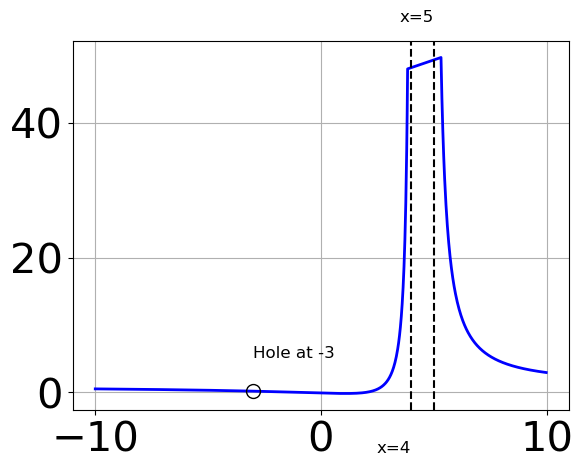
\includegraphics[width=0.5\textwidth]{../Figures/identifyGraphOfRationalFunctionCopyB.png}
\end{center}
\begin{enumerate}[label=\Alph*.]
\item \( f(x)=\frac{x^{3} -2.0 x^{2} -x + 2.0}{x^{3} -6.0 x^{2} -7.0 x + 60.0} \)
\item \( f(x)=\frac{x^{3} +2.0 x^{2} -5.0 x -6.0}{x^{3} -6.0 x^{2} -7.0 x + 60.0} \)
\item \( f(x)=\frac{x^{3} -2.0 x^{2} -5.0 x + 6.0}{x^{3} +6.0 x^{2} -7.0 x -60.0} \)
\item \( f(x)=\frac{x^{3} -4.0 x^{2} -7.0 x + 10.0}{x^{3} +6.0 x^{2} -7.0 x -60.0} \)
\item \( \text{None of the above are possible equations for the graph.} \)

\end{enumerate} }
\litem{
Determine the horizontal and/or oblique asymptotes in the rational function below.\[ f(x) = \frac{12x^{3} -5 x^{2} -43 x + 30}{3x^{2} -20 x + 25} \]\begin{enumerate}[label=\Alph*.]
\item \( \text{Horizontal Asymptote of } y = 4.0  \)
\item \( \text{Horizontal Asymptote of } y = 5.0 \text{ and Oblique Asymptote of } y = 4x + 25 \)
\item \( \text{Horizontal Asymptote at } y = 5.0 \)
\item \( \text{Oblique Asymptote of } y = 4x + 25. \)
\item \( \text{Horizontal Asymptote of } y = 4.0 \text{ and Oblique Asymptote of } y = 4x + 25 \)

\end{enumerate} }
\litem{
Determine the horizontal and/or oblique asymptotes in the rational function below.\[ f(x) = \frac{12x^{3} -35 x^{2} +33 x -10}{4x^{2} +7 x -15} \]\begin{enumerate}[label=\Alph*.]
\item \( \text{Horizontal Asymptote of } y = -3.0 \text{ and Oblique Asymptote of } y = 3x -14 \)
\item \( \text{Horizontal Asymptote at } y = -3.0 \)
\item \( \text{Oblique Asymptote of } y = 3x -14. \)
\item \( \text{Horizontal Asymptote of } y = 3.0 \text{ and Oblique Asymptote of } y = 3x -14 \)
\item \( \text{Horizontal Asymptote of } y = 3.0  \)

\end{enumerate} }
\litem{
Determine the horizontal and/or oblique asymptotes in the rational function below.\[ f(x) = \frac{30x^{3} -47 x^{2} -114 x -45}{10x^{3} +22 x^{2} -42 x -18} \]\begin{enumerate}[label=\Alph*.]
\item \( \text{Horizontal Asymptote of } y = 3.000  \)
\item \( \text{Horizontal Asymptote of } y = 0  \)
\item \( \text{Vertical Asymptote of } y = 3  \)
\item \( \text{Vertical Asymptote of } y = -1.000  \)
\item \( \text{None of the above} \)

\end{enumerate} }
\litem{
Determine the vertical asymptotes and holes in the rational function below.\[ f(x) = \frac{6x^{3} -7 x^{2} -7 x + 6}{6x^{2} +5 x -6} \]\begin{enumerate}[label=\Alph*.]
\item \( \text{Holes at } x = -1.5 \text{ and } x = 0.667 \text{ with no vertical asymptotes.} \)
\item \( \text{Vertical Asymptotes of } x = -1.5 \text{ and } x = 0.667 \text{ with no holes.} \)
\item \( \text{Vertical Asymptote of } x = 1.0 \text{ and hole at } x = 0.667 \)
\item \( \text{Vertical Asymptote of } x = -1.5 \text{ and hole at } x = 0.667 \)
\item \( \text{Vertical Asymptotes of } x = -1.5 \text{ and } x = 1.5 \text{ with a hole at } x = 0.667 \)

\end{enumerate} }
\litem{
Determine the horizontal and/or oblique asymptotes in the rational function below.\[ f(x) = \frac{3x^{2} -17 x + 10}{15x^{3} -58 x^{2} -16 x + 32} \]\begin{enumerate}[label=\Alph*.]
\item \( \text{Horizontal Asymptote at } y = 5.000 \)
\item \( \text{Horizontal Asymptote of } y = 0 \)
\item \( \text{Horizontal Asymptote of } y = 0.200 \text{ and Oblique Asymptote of } y = 5x + 9 \)
\item \( \text{Oblique Asymptote of } y = 5x + 9. \)
\item \( \text{Horizontal Asymptote of } y = 0.200  \)

\end{enumerate} }
\litem{
Which of the following functions \textit{could} be the graph below?
\begin{center}
    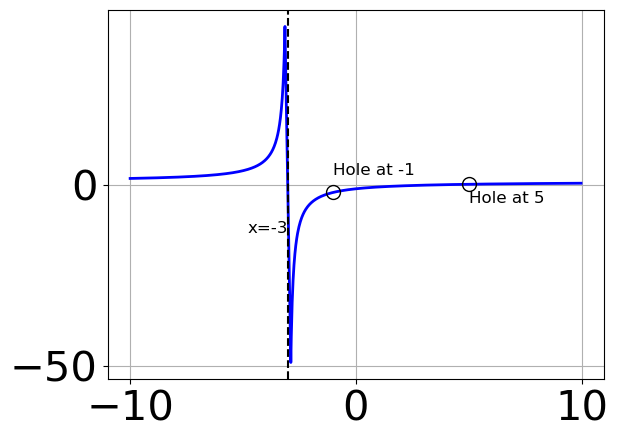
\includegraphics[width=0.5\textwidth]{../Figures/identifyGraphOfRationalFunctionB.png}
\end{center}
\begin{enumerate}[label=\Alph*.]
\item \( f(x)=\frac{x^{3} +7.0 x^{2} +7.0 x -15.0}{x^{3} + x^{2} -17.0 x + 15.0} \)
\item \( f(x)=\frac{x^{3} + x^{2} -24.0 x + 36.0}{x^{3} -1.0 x^{2} -17.0 x -15.0} \)
\item \( f(x)=\frac{x^{3} -6.0 x^{2} -7.0 x + 60.0}{x^{3} + x^{2} -17.0 x + 15.0} \)
\item \( f(x)=\frac{x^{3} -7.0 x^{2} +7.0 x + 15.0}{x^{3} -1.0 x^{2} -17.0 x -15.0} \)
\item \( \text{None of the above are possible equations for the graph.} \)

\end{enumerate} }
\litem{
Determine the vertical asymptotes and holes in the rational function below.\[ f(x) = \frac{6x^{3} +13 x^{2} -9 x -10}{12x^{2} +23 x + 10} \]\begin{enumerate}[label=\Alph*.]
\item \( \text{Vertical Asymptotes of } x = -1.25 \text{ and } x = -2.5 \text{ with a hole at } x = -0.667 \)
\item \( \text{Vertical Asymptote of } x = 0.5 \text{ and hole at } x = -0.667 \)
\item \( \text{Vertical Asymptotes of } x = -1.25 \text{ and } x = -0.667 \text{ with no holes.} \)
\item \( \text{Vertical Asymptote of } x = -1.25 \text{ and hole at } x = -0.667 \)
\item \( \text{Holes at } x = -1.25 \text{ and } x = -0.667 \text{ with no vertical asymptotes.} \)

\end{enumerate} }
\end{enumerate}

\end{document}